% ********** Chapter 1 **********
\section{Design}
\label{sec:chap1:design}

Eine JSR 223 Implementation f"ur PHP besteht gezwungenermassen aus zwei Teilen: einem Java-Teil, welcher im Wesentlichen
die ScriptEngineFactory enth"alt, komplett in Java ohne die Verwendung von nativen (JNI-) Aufrufen implementiert ist und
s"amtliche Funktionalit"at des Auffindungsmechanismus abdeckt, sowie einem nativen Teil, welcher aus 
einem C- oder C++ - Programm das die n"otigen Aufrufe an PHP vornimmt und der eigentlichen ScriptEngine besteht, die dieses in
nativen Code "ubersetzte Programm mittels JNI anspricht. TODO: Arschlochsatz
Um allerdings JSR 223 "uberhaupt nutzen zu k"onnen m"ussen die Klassen aus javax.script, vor allem der ScriptEngineManager, 
im Java-Classpath liegen. Hierzu kann entweder eine Java-Runtime der Version 6, oder aber eine eigene Implementation dieser
Klassen genutzt werden. Wichtige Use-Cases f"ur diesen Teil des Projektes sind:
\begin{enumerate}
\item Test, ob die PHP-ScriptEngine verf"ugbar ist. Durch einfache Ausgabe auf der Konsole soll schnell ermittelbar sein, welche
    ScriptEngines geladen und einsatzbereit sind. Dies dient haupts"chlich der "Uberpr"ufung, ob die aktuelle Java-Umgebung
    richtig konfiguriert ist.
\item Test, ob die PHP-ScriptEngine funktioniert. Es soll ein einfaches PHP-Skript ausgef"uhrt werden, um dem Anwender
    die korrekte Funktionsweise der ScriptEngine vorzuf"uhren und zu pr"ufen ob die nativen Teile der Implementation
    ordnungsgem"a\ss funktionieren.
\item Ausf"uhren beliebiger PHP-Skripte. Es soll dem Anwender m"oglich sein, ohne selbst Java-Quelltext zu schreiben, beliebige
    PHP-Skripte auszuf"uhren.
\end{enumerate}
Die im folgenden beschriebene JSR 223 Implementation tr"agt den Namen "'Turpitude"'.

\subsection{Java}
\label{sec:chap1:design:java}

Um f"ur ScriptEngineManager auffindbar zu sein muss eine JSR 223 Implementation sich gem"ass der \emph{Jar File Specification} \cite{JARSPEC} 
als sogenannter \emph{Service Provider} registrieren. Hierzu muss sich im Verzeichnis \emph{META-INF/services} des .jars eine Datei
mit dem Namen der Service-Klasse (in diesem Fall \emph{javax.script.ScriptEngineFactory}) befinden, in welcher verf"ugbare 
ScriptEngineFactories zeilenweise aufgelistet werden.

Alle Klassen der Implementation befinden sich im Package \emph{net.xp\_framework.turpitude}. 
Die ScriptEngineFactory-Implementation hei\ss t \emph{PHPScriptEngineFactory} und implementiert direkt das Interface 
\emph{ScriptEngineFactory} aus \emph{javax.script}. Im Gegensatz dazu implementiert die Klasse \emph{PHPScriptEngine} nicht
direkt das Interface \emph{ScriptEngine}, sondern erbt von der abstrakten Klasse \emph{AbstractScriptEngine}, welche f"ur
viele Varianten der \emph{eval()}-Methode schon eine Realisierung, sowie mit der Klasse \emph{SimpleScriptContext} schon einen 
\emph{ScriptContext} mitbringt. Um den "ubergebenen Scriptcode tats"achlich auszu"fuhren muss dieser an den mittels der Java-Methode
\emph{System.loadLibary()} geladenen nativen Teil der Implementation weitergegeben werden. Die Kommunikation mit diesem
nativen Teil findet mittels der JNI-Methoden TODO: Methoden auflisten.
Die Abbildung \ref{fig:jsr223impl} zeigt die beteiligten Klassen und ihre Abh"anigkeiten untereinander,
zusammen mit einigen wichtigen Methoden und Attributen. 

\begin{figure}[h]
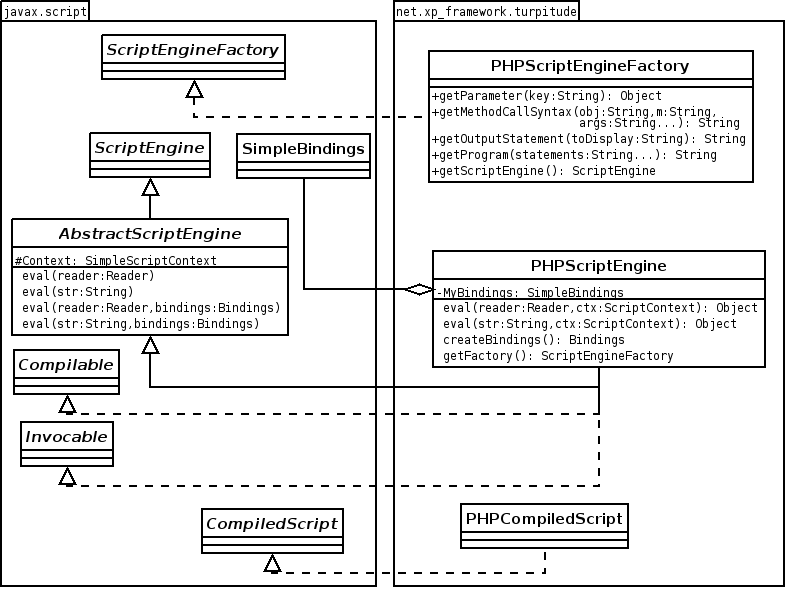
\includegraphics[width=\textwidth]{chap1/img/turpitude.png}
\caption{JSR 223 Implementation - Architektur}
\label{fig:jsr223impl}
\end{figure}

TODO: Compilable, Invocable
TODO: Use-Cases

\subsection{Native}
\label{sec:chap1:design:native}

Der native Teil der Implementation teilt sich wiederum auf in JNI-Methoden, f"ur welche die Headerdateien automatisch aus
der Java-Klasse der PHPScriptEngine generiert werden k"onnen, und in die Implementation einer SAPI. Hierzu muss im
Wesentlichen ein sogenanntes \emph{sapi\_module\_struct} angelegt und bef"ullt werden, welches neben einigen Strings
haupts"achlich Funktionspointer auf R"uckruffunktionen enth"alt, welche vom PHP-Interpreter aufgerufen werden. Da es
kaum m"oglich ist dieses Konstrukt sinnvoll in eine objektorientierte Architektur einzuf"ugen, wird auf eine solche
vollst"andig verzichtet. Das sapi\_module\_struct und die dazugeh"origen Funktionen werden in traditioneller,
prozeduraler Art und Weise implementiert.
TODO: JNI Methoden
TODO: sapi methoden






% ********** End of chapter **********
